\lecture{11}{8. april 2025}{Varmepumper og Kølemaskiner}

\section{Kølemaskiner og varmepumper}
Kølemaskiner og varmepumper er grundlæggende baseret på samme kredsprocess. Fokusset for de to maskiner er dog forkskellige idet den ene søger mod at køle, medens den anden forsøger at varme.

\subsection{Kølekredsprocessen}
Carnots arbejdskonsumerende kredsproces er egentligt blot en idealiseret kølekredsproces. Carnots kredsproces er teoretisk og der ville blandt andet være problemer i den isentropiske kompression mellem tilstand 2 og 3 da en kompressor ikke kan arbejde effektivt i tofaseområdet, da væskedelen vil lave ``væskeslag'' hvilket både forringer kompressorens effektivitet og ydeevne. I virkeligheden er processen derfor istedet:
\begin{itemize}
  \item \textbf{Tilstand 1-2}: Delvis isotermisk varmetilførsel (fordamper)
  \item \textbf{Tilstand 2-3}: Isentropisk kompression (kompressor)
  \item \textbf{Tilstand 3-4}: Delvis isotermisk varmeafgivelse (kondenser)
  \item \textbf{Tilstand 4-1}: Isentalpisk ekspansion (drøvleorgan)
\end{itemize}
Det bør dog nævnes at dette også er en idealisering. I virkeligheden vil den isetropiske virkningsgrad af kompressoren forårsage at den egentlige processvej mellem tilstand 2 og 3 stiger hurtigere i entalpi end den tilvarende isentroplinje, hvilket også kan ses på \textbf{\autoref{fig:f11_1}}.

\begin{figure} [ht]
  \centering
  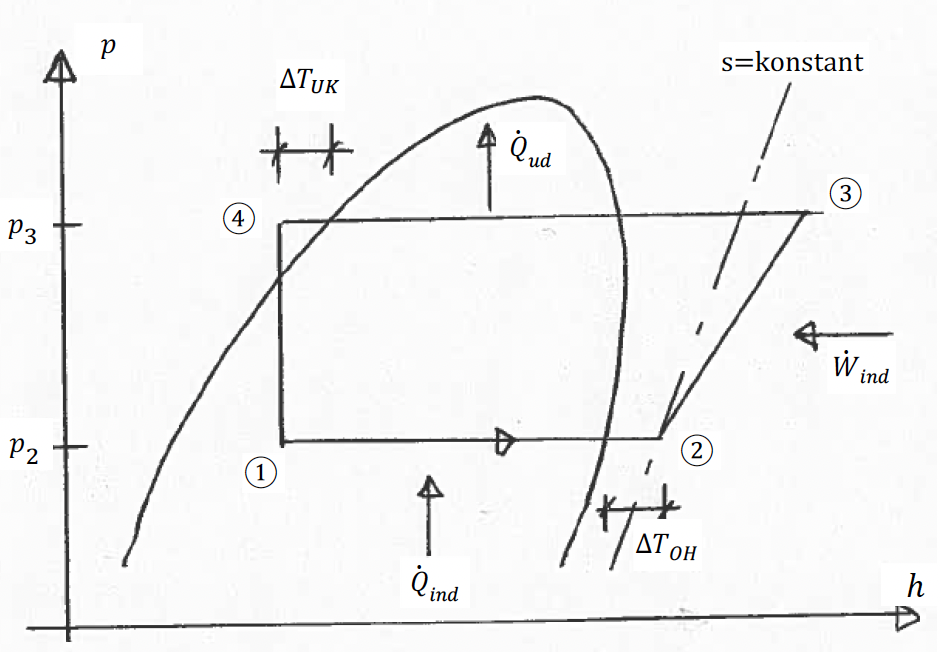
\includegraphics[width=0.5\linewidth]{./figures/f11_1.png}
  \caption{Kølekredprocessen i et $p$-$h$ diagram}
  \label{fig:f11_1}
\end{figure}

Af \textbf{\autoref{fig:f11_1}} ses også at kølekredsprocessen opererer mellem to trykniveauer. Ved det lave trykviveau ($p_2 = p_1$) fordamper kølemidlet ved en lav temperatur, hvorved et andet medie (eksempelvis indeluft) kan køles. Ved det høje trykniveau ($p_4=p_3$) kondenserer kølemidlet ved en temperatur, som muliggør, at varmen kan overføres til et andet medie (eksempelvis udeluft).

På \textbf{\autoref{fig:f11_1}} er også anført en størrelse kaldet $\Delta T_{\mathrm{OH}}$ der angiver temperaturforskellen mellem mætningstemperaturen ved fordampningstrykket og den reelle gastemperatur idet den kommer ind i kompressoren. Denne størrelse kaldes overhedningen og sikrer mod at der kommer væskedråber i kompressoren.

Ligeledes kaldes størrelsen, $\Delta T_{\mathrm{UK}}$ for underkølingen. Denne angiver forskellen mellem mætningstemperaturen og den relle gastemperatur ved afgang fra kondenseren. Denne sikrer at ingen gasbobler ledes videre til drøvleorganget. Dannelse af gasbobler efter kondenseren kaldes i fagsprog ``\textit{flashgas}''.

\begin{figure} [ht]
  \centering
  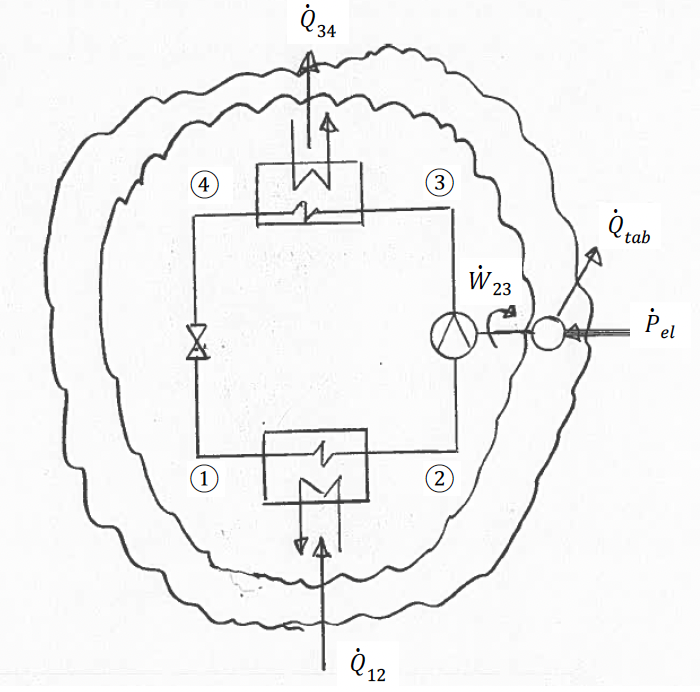
\includegraphics[width=0.4\linewidth]{./figures/f11_2.png}
  \caption{Procesdiagram for kølekredsproces}
  \label{fig:f11_2}
\end{figure}

På \textbf{\autoref{fig:f11_2}} er indtegnet et procesdiagram for en kølekredsproces. Med afsæt i denne kan følgende to formål opstilles:
\begin{itemize}
  \item \textbf{Kølemaskine (indeks R)}: Formålet er at aftage energi fra lavtemperaturreservoiret og ``ønsket energimængde'' er derfor $\dot{Q}_{\mathrm{ind}}=\dot{Q}_{12}$.
  \item \textbf{Varmepumpe (indeks HP)}: Formålet er at levere energi til højtemperaturreservoiret og ``ønsket energimængde'' er derfor $\dot{Q}_{\mathrm{ud}}=\dot{Q}_{34}$.
\end{itemize}

På \textbf{\autoref{fig:f11_2}} er også indtegnet to systemgrænser. Hvis det antages at tab i gear, motor og mekaniske tab tilflyder omgivelserne benyttes den indre af de to og hvis det antages at de førnævnte tab tilflyder kølemidlet benyttes den ydre af de to. For hver systemgrænse kan opstilles en formel for $\mathrm{COP}$-faktorerne af hhv. køleaskiner og varmepumper:

\paragraph{Indre systemgrænse}:
\begin{align*}
  \mathrm{COP}_{\mathrm{R}} &= \frac{\left| \dot{Q}_{\mathrm{ind}} \right|}{\left| \dot{W}_{\mathrm{net}} \right|} = \frac{\dot{Q}_{12}}{\dot{W}_{23}} \\
  \mathrm{COP}_{\mathrm{HP}} &= \frac{\left| \dot{Q}_{\mathrm{ud}} \right|}{\dot{W}_{\mathrm{net}}} = \frac{\left| \dot{Q}_{34} \right|}{\dot{W}_{23}}
.\end{align*}

\paragraph{Ydre systemgrænse}:
\begin{align*}
  \mathrm{COP}_{\mathrm{R, ydre}} &= \frac{\left| \dot{Q}_{\mathrm{ind}} \right|}{\left| \dot{P}_{\mathrm{el}} \right|} = \frac{\dot{Q}_{12}}{\dot{P}_{\mathrm{el}}} \\
  \mathrm{COP}_{\mathrm{HP, ydre}} &= \frac{\left| \dot{Q}_{\mathrm{ind}} \right|}{\left| \dot{P}_{\mathrm{el}} \right|} = \frac{\left| \dot{Q}_{34} \right|}{\dot{P}_{\mathrm{el}}}
.\end{align*}

De indre COP-faktorer er mest anvendt i den klassiske termodynamik mens de ydre er mere anvendelige i virkeligheden idet de angiver en direkte sammenhæng imellem leveret varmemængde og elforbrug. Værd at bemærke er også at de ydre COP-faktorer vil være mindre end de indre, da eleffekten $\dot{P}_{\mathrm{el}}$ er større end akseleffekten $\dot{W}_{23}$. 

Desuden gælder følgende sammenhæng mellem COP-faktorerne for den indre systemgrænse:
\[ 
\mathrm{COP}_{\mathrm{HP}} = \mathrm{COP}_{\mathrm{R}} + 1
.\]


\subsection{Kølemidler}
Midlet der cirkulerer i en kølekreds kaldes \textit{kølemidlet} eller en \textit{refrigerant} i engelsksproget litteratur. Kølemidler grupperes overordnet set i syntetiske, organiske og naturlige kølemidler.

Kølemidler vurderes på deres miljøpåvirkning, herunder ODP som står for \textit{Ozone Depletion Potential} dvs. bidrag til reduktion af ozonlaget samt GWP som står for \textit{Global Warming Potential}, dvs. bidrag til global opvarmning.

Anvendelsen af de forskellige kølemidler indebærer forskellige fordele og ulemper, og af ulemper skal specielt fremhæves giftigvirkning på flora of fauna, brandfare, eksplosionsfare og arbejdsmiljø-relaterede aspekter. Generelt bør an stille følgende krav til det ideelle kølemiddel:
\begin{enumerate}
  \item Prisvenlig
  \item Lav ODP og GWP
  \item Ikke-skadeligt for flora og fauna
  \item Lav arbejsmiljøbelastning
  \item Ikke brændbart
  \item Kemisk stabilt
  \item Ikke at reagere med smøreolie og anlægsmaterialer
  \item Resultere i høj COP-faktor
  \item Give anledning til et moderat kondenseringstryk
  \item Give anledning til et fordampningstryk > 1 bara ved drift
\end{enumerate}
På \textbf{\autoref{fig:f11_3}} er anført en række kølemidler og deres ODP og GWP.
\begin{figure} [ht]
  \centering
  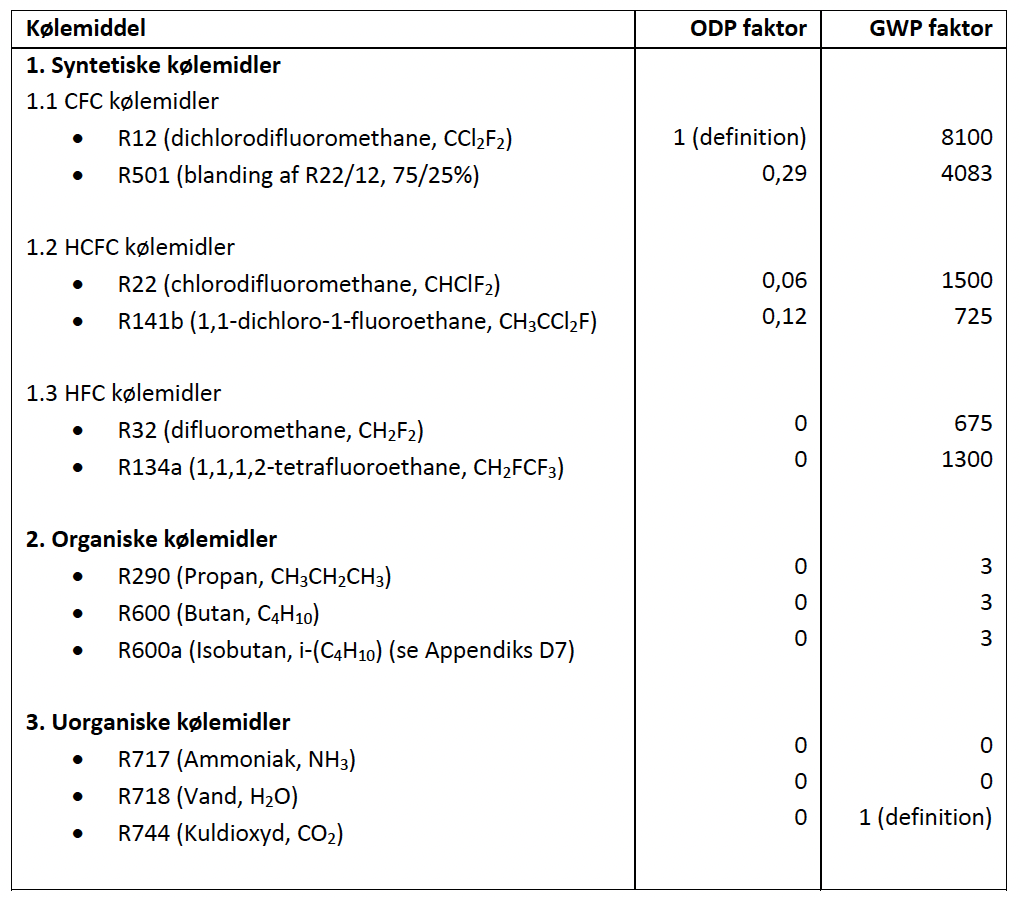
\includegraphics[width=0.3\linewidth]{./figures/f11_3.png}
  \caption{Gruppeinddeling af kølemidler og miljøfaktorer}
  \label{fig:f11_3}
\end{figure}

Vand ($\mathrm{H}_2 \mathrm{O}$/R718) er i mange situationer et godt valg, men man skal huske at det ikke er velegnet til temperaturer under \qty{0}{\celsius} da det her går på fast form. Ammoniak ($\mathrm{NH}_3$/R717) er også hyppigt brugt. Dog er ammoniak giftigt, brændbart, eksplosivt og arbejdsmiljøskadeligt. I de senere år er man også begyndt at bruge kuldioxid ($\mathrm{CO}_2$/R744) som kølemiddel.


\subsection{Optimering af kredsprocessen}
\subsubsection{Ét-trins anlæg}
Trykforskel mellem lav- og højtrykssiden har stor indflydelse på effektforbruget på kompressoren (se evt. definitionen af teknisk arbejde: $\dot{W}_t = \dot{m} \cdot \int_{1}^{2} v \cdot \mathrm{d}p$). Trykforskellen indgår direkte i formlen og det er klart at en indre trykforskel giver et mindre effektforbrug til kompression af kølemidlet.

Trykforskellen mellem lav- og højtrykssiden kan reduceres enten ved at forhøje fordampningstrykket eller ved at mindske kondenseringstrykket. Disse er imidlertid ofte bestemt af funktionskrav såsom ønsket temperatur i et fryserum og brug af udeluft til køling af kondenseren.

Et større varmeoverførende areal i en varmeveksler giver en bedre varmeoverføresel, hvorfor en temperaturforskel i så fald kan mindskes. Dette giver en marginal øgning af fordampningstrykket hvilket giver en bedre COP-faktor og et lavere effektforbrug til kompressoren. Her skal man altså afveje øgede anlægsomkostninger mod lavere driftsomkostninger.

Som tomelfingerregel benytter man det eksterne kølemedium i kondenseren der har den laveste temperatur. Dette giver et lavere kondenseringstryk og dermed en bedre COP-faktor. Derved opstår et dilemma når man skal vælge mellem eksempelvis luft og havvand, da havvand ofte er koldere om sommeren mens luften typisk er koldere om vinteren.

Derudover kan det vises at en større underkøling også giver en bedre COP-faktor.

\subsubsection{To-trins anlæg med mellemkøling}
I visse situationer kan det være en fordel at udføre kompressionen i to trin. For anlæg med en stor trykforskel kan det ligefrem være nødvendigt da temperaturen på kølemidlet ellers ville blive for høj under kompressionen.

En af fordelene der opnås ved at gøre det på denne måde er at man får mulighed for at køle kølemiddelgassen mellem de to kompressorer. Dette kaldes mellemkøling.

Med reference til definitionen på det teniske arbejde $\dot{W}_t = \dot{m} \int_{1}^{2} v \, \mathrm{d}p$ ses også at en underkøling giver et mindre specifikt volumen hvilket giver et mindre arbejde end for den tilsvarende ikke-mellemkølede process.

Mellemkøling kan opnås i forskellige anlægstyper. Eksempelvis kan mellemkølingen opnås ved at lade den overhedede kølemiddelgas fra kompressor 1 boble op gennem kølemiddelvæsken i mellemkøleren. Herved køles kølemiddelgassen ned til mætningstemperaturen ved trykket i mellemkøleren eller til tilstand $h'' (x=1)$. Kølemiddelgassen før kompressor 2 er således uden overhedning.
